\section{Evaluation}
\label{sec:eval}

We evaluate Defense~4 on a testbed with a physical master, one Tofino-1, and a physical SEL-751 relay.
Native and defended traffic are captured on the same loaded binary, separated only by a runtime mode
change, so the comparison isolates the defense. The defended captures carry no TCP timestamp option.
The analysis regenerates deterministically from the traces, and a manifest verifies every derived
artifact.

\noindent\textbf{Timing.} The native CLRT median is 1.272~ms for read (mean 1.880, standard deviation
1.354, $n{=}999$) and 2.107~ms for select ($n{=}488$), with heavy tails. The defended CLRT median is
4.001~ms for both classes, with standard deviation 0.022~ms (read) and 0.021~ms (select), matching the
policy $R-A=4$~ms; the master-facing offsets of about 21 and 25~ms include a documented path and
capture offset of roughly 1~ms over the configured 20 and 24~ms. Defense~4 adds 2.73~ms to a read and
1.89~ms to a select.

\noindent\textbf{Segment shape and reconstruction.} The native read is a single 49-byte segment. All
1{,}280 defended eligible responses (600 read, 500 select, and 90 select and 90 operate from the
control transactions) present the $[28,21]$ segment vector. Each reconstruction is
sequence-contiguous, DNP3-block-CRC-valid, and IP/TCP-checksum-valid, and no defended response escapes
as an unsplit 49-byte segment. Because no paired source-side capture exists, we report a CRC-valid
49-byte reconstruction rather than byte identity to a source frame.

\noindent\textbf{Control-command timing.} Figure~\ref{fig:timeline} shows the master-facing ACK and
echo placement for a control command. The echo-minus-ACK gap is 4.00~ms and does not vary with the
internal release delay: across $J\in\{2,6,12\}$~ms the pooled gap median is 4.002~ms with standard
deviation 0.026~ms ($n{=}90$).

\begin{figure}[t]
\centering
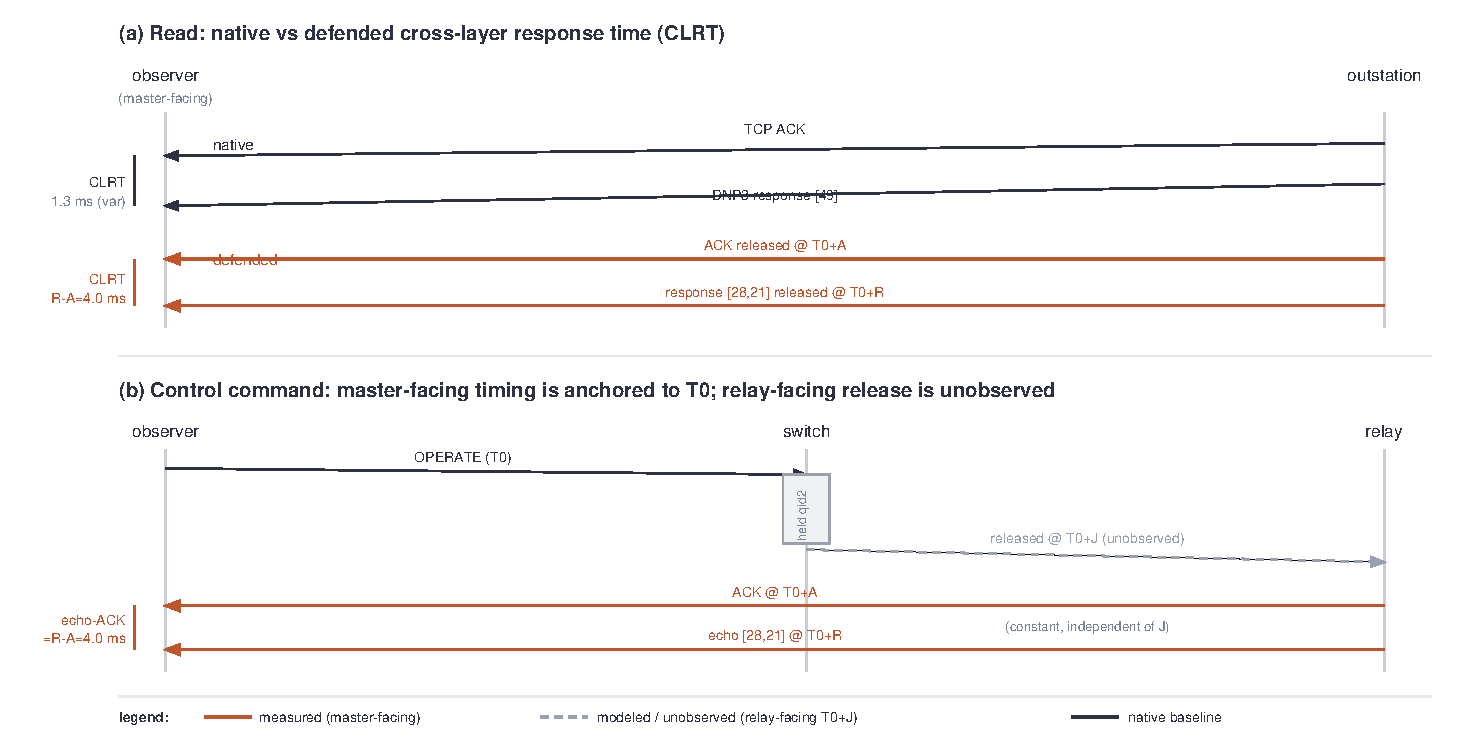
\includegraphics[width=0.98\columnwidth]{figures/fig_timeline}
\caption{Master-facing timing of a control command. The ACK and echo are placed at $T_0{+}A$ and
$T_0{+}R$, anchored to the OPERATE arrival $T_0$, so the observable gap $R-A$ is fixed. The internal
release at $T_0{+}J$ is on the relay-facing link and is not captured (dashed), so it is verified by the
implementation model rather than measured.}
\label{fig:timeline}
\end{figure} The
relay-facing release time and the number of copies delivered to the relay are not captured; the
offline model verifies the single release at $T_0{+}J$, and the captures establish that the master
issued one OPERATE per transaction.

\noindent\textbf{Fingerprint suppression.} We quantify the leak with mutual information between the
transaction class and the CLRT, using common bins and a permutation null. The native mutual information
is 0.424~bits, well above the null band, and the defended value is 0.0018~bits, inside it. A logistic
classifier trained to separate read from select by CLRT reaches 0.592 balanced accuracy on native
traffic and 0.500, the chance baseline, on defended traffic. This is a transaction-class task on one
device, not a device-identity task; Defense~4 replaces the evaluated CLRT and segment-shape features
for the SEL-751 rather than establishing indistinguishability among devices.

\noindent\textbf{Safety and resource fit.} The guarded control test permitted only the isolated CROB
points $\{1,3\}$ and refused the breaker-close index~6; all 32 relay outputs remained OPEN throughout,
and no breaker operation was attempted. The program compiles for one Tofino-1 ingress pipe within the
twelve-stage budget.

\section{Discussion}
\label{sec:disc}

Defense~4 replaces two master-facing features of one outstation with a fixed policy and preserves the
protocol. It does not hide the total 49-byte payload length, which a full TCP reassembler recovers,
and it does not establish multi-device anonymity or resistance to every traffic-analysis feature.
Extending the eligible class beyond the 49-byte responses would require a segment-vector policy for
each response size, which the CRC-block structure supports but we have not evaluated. The strongest
open item is relay-facing verification: a tap on the relay-facing link would turn the modeled
single-release property into a measured one, and we leave this instrumentation to future work.

\section{Conclusion}
\label{sec:concl}

We presented Defense~4, an in-network defense that normalizes the cross-layer response time and the
TCP segment shape of DNP3 traffic in the data plane of one programmable switch, without modifying a
DNP3 byte or recomputing a CRC. A timing primitive releases the ACK and response at fixed offsets from
the request, a replication-and-carving path fixes the eligible segment vector at an existing CRC
boundary, and a control-command primitive hides operation timing while anchoring the master-visible
acknowledgment to the request. On a physical SEL-751 relay, the defense normalizes the defended CLRT to
4.001~ms, presents every eligible response as $[28,21]$ with a CRC-valid reconstruction, holds the
control-command gap at 4.00~ms across release delays, and drives a read-versus-select timing classifier
to chance, within a stated single-device and master-facing evaluation boundary.
